% coding:utf-8

\section{Layout}
Die Platine wird direkt an den XLR-Stecker vom Typ NC3MD-V von Neutrik angel�tet. Die Verbindung zu einem Arduino erfolgt �ber eine Steckerleiste. Alle �brigen Bauteile sind in SMD mit der Baugr�sse 0805 bzw. 1206 ausgef�hrt. Die Gr�sse der Platine ist auf den Steckverbinder angepasst, so dass dieser mit der angel�teten Platine montiert werden kann. 
\begin{figure}[h!]
	\centering
	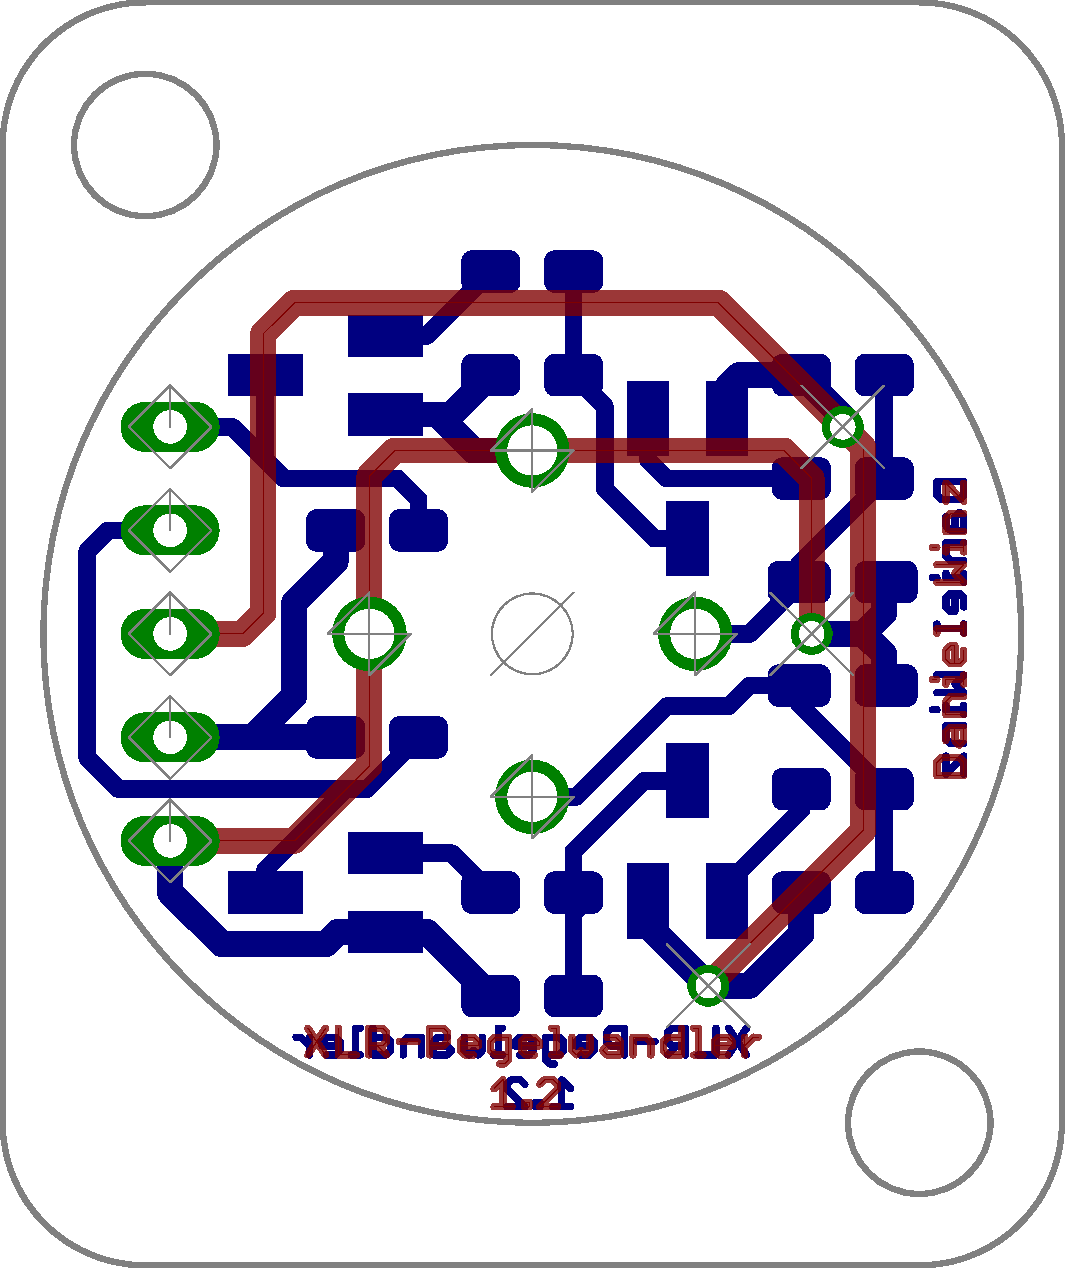
\includegraphics[scale=\layscale]{fig/xlr_pegelwandler_v_1_2_lay_transp.pdf}
	\caption{Layout}
	\label{lay:pegw}
\end{figure}
